\newcommand{\tspr}{~$TSPR$~}

%%%%%%%%%%%%%%%%
\section{课题背景及意义}
\label{Introduction:background}
%%%%%%%%%%%%%%%%%%%%%%%%%%%%%%%%%%%%%%%%%%%%%%%%%%%%%

\subsection{课题背景}
\label{sec:back}

\frame{
\frametitle{太极拳背景介绍}
\begin{itemize}
\item 太极拳好~\cite{taiji}~
\item 太极拳非常好
\end{itemize}
{\alert{本课题来源于于国家~863~项目:太极拳和三个代表(No. 123456789)}}


}

%%%%%%%%%%%%%%%%%%%%%%%%%%%%%%%%%%%%%%%%%%%%%%%%%%%%%
\frame{
\frametitle{太极拳无敌}
\begin{center}
 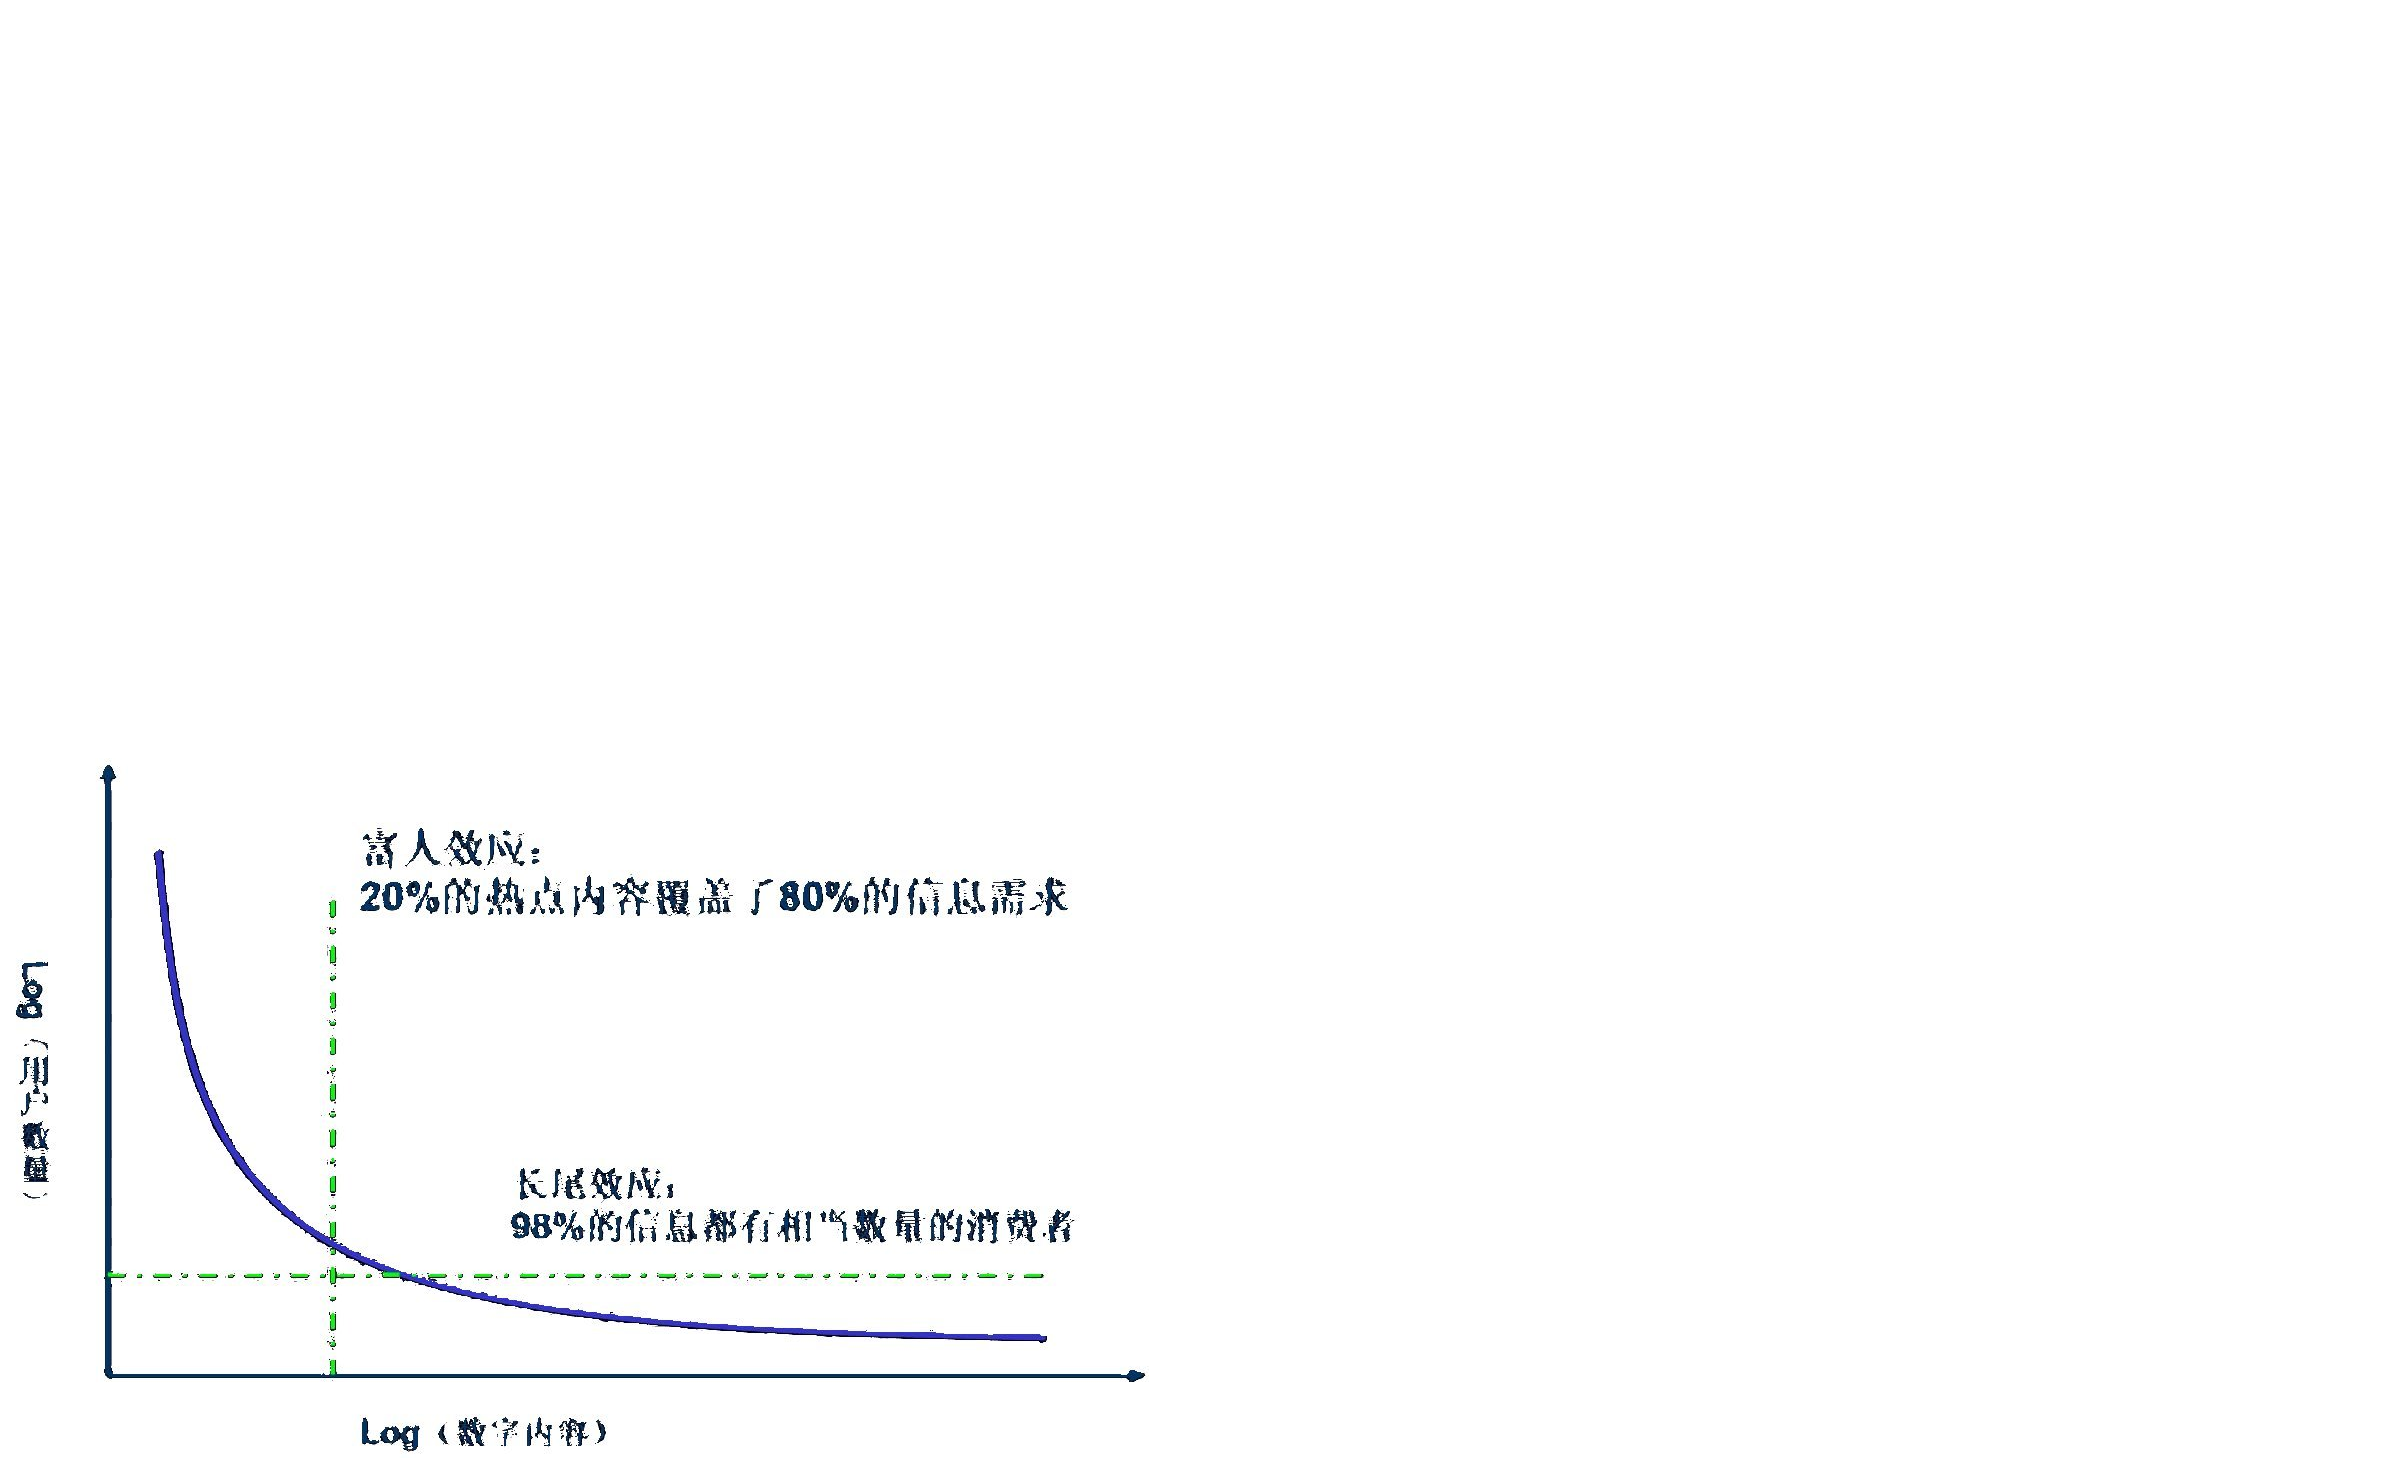
\includegraphics[height=2.5cm]{long-tail.pdf}
\end{center}
\begin{itemize}
\item 太极包容一切
\item 太极代表一切
\end{itemize}
}

%%%%%%%%%%%%%%%%%%%%%%%%%%%%%%%%%%%%%%%%%%%%%%%%%%%%%

\subsection{研究意义}
\label{sec:means}

\frame{
\frametitle{研究的意义}
\begin{itemize}
\item 意义
\end{itemize}
}

%%%%%%%%%%%%%%%%%%%%%%%%%%%%%%%%%%%%%%%%%%%%%%%%%%%%%
\section{国内外研究现状分析}
\label{sec:researchsituation}
%%%%%%%%%%%%%%%%%%%%%%%%%%%%%%%%%%%%%%%%%%%%%%%%%%%%%
\frame{
\frametitle{太极独步天下}

\begin{itemize}
\item 无人能敌
\item 暂不外传
\end{itemize}
}

\section{主要研究内容和方案}
\label{sec:researchplan}
%%%%%%%%%%%%%%%%%%%%%%%%%%%%%%%%%%%%%%%%%%%%%%%%%%%%%
\frame{
\frametitle{总体研究思路}
}
 

\subsection{太极剑}
\label{sec:topic_crawler}
%%%%%%%%%%%%%%%%%%%%%%%%%%%%%%%%%%%%%%%%%%%%%%%%%%%%%
 
%%%%%%%%%%%%%%%%%%%%%%%%%%%%%%%%%%%%%%%%%%%%%%%%%%%%%
\frame{
\frametitle{太极剑研究内容}
见于相关论文的方法主要有以下几种:
\begin{itemize}
\item 基于“内功”的方法
\item 基于“招式”方法。
\item 其他方法
\end{itemize}

}
%%%%%%%%%%%%%%%%%%%%%%%%%%%%%%%%%%%%%%%%%%%%%%%%%%%%%
\frame[allowframebreaks]{
\frametitle{常用链接分析方法}
最为有效的两种传统方法是PageRank~\cite{pagerank}~和HITS~\cite{hits}~。

PageRank方法是~L. Page~和~S. Brin~于1998年提出的基于网络链接分析对网页
排序的方法。最初是用来对搜索引擎返回的结果页面进行排序,以完成网页的自
动排名和提高搜索引擎的服务质量。
一些相关定义:
\begin{definition}{$I(v)$~:}
  网页~$v$~的入度。即,指向网页~$v$~的网页数目
\end{definition}
\begin{definition}{$O(v)$~:}
网页~$v$~的出度,即网页指向~$v$~的网页数目
\end{definition}
\begin{definition}{$N$~ :}
网页集合~$W$~的网页数量
\end{definition}
\begin{definition}{ $d$~ :}
在随机浏览模型中,用户从一个网页随机跳到另外一个网页的概率
\end{definition}
\begin{definition}{$p\rightarrow q$ :}
存在从网页~$p$~到网页 ~$q$~的一个超链接
\end{definition}
令~$PR(i)$~表示网页~$i$~的排序值,则最基本的PageRank~方法可以形式化描述如下:
\begin{equation}
  \label{eq:page-rank}
  PR(i)=(1-d) \sum_{j:j \rightarrow i}{\frac{ PR(j)}{O(j)} }+d\frac{1}{N}
\end{equation}

}
%%%%%%%%%%%%%%%%%%%%%%%%%%%%%%%%%%%%%%%%%%%%%%%%%%%%%


\subsection{太极脚}
\label{sec:web_social}
%%%%%%%%%%%%%%%%%%%%%%%%%%%%%%%%%%%%%%%%%%%%%%%%%%%%%

\section{前期研究与试验工作}
\label{sec:prework}


\subsection{太极起步阶段}
\label{sec:step}
%%%%%%%%%%%%%%%%%%%%%%%%%%%%%%%%%%%%%%%%%%%%%%%%%%%%%
\frame{
\frametitle{太极起步}
\begin{figure}[htbp]
\centering
  
\includegraphics[width = 3cm]{golfer.pdf}
\label{Figure:research}
\end{figure}

}
%%%%%%%%%%%%%%%%%%%%%%%%%%%%%%%%%%%%%%%%%%%%%%%%%%%%%



\section{论文进度安排和预期目标}
\label{sec:destination}
%%%%%%%%%%%%%%%%%%%%%%%%%%%%%%%%%%%%%%%%%%%%%%%%%%%%%
\frame{
\frametitle{已经完成的工作}
\begin{itemize}
\item 太极1
\item 太极2
\end{itemize}
}
%%%%%%%%%%%%%%%%%%%%%%%%%%%%%%%%%%%%%%%%%%%%%%%%%%%%%
\frame[allowframebreaks]{
\frametitle{时间安排}
拟定工作时间从xxxx年x月至明xxxx年xx月,初步安排如下:
\begin{itemize}
\item xx年x月-x月:进一步完善太极拳
\item xx年x月-x月:进一步完善太极剑
\item xx年x月-x月:进一步完善太极脚
\item xx年x月:开始撰写毕业论文
\end{itemize}

}

%%%%%%%%%%%%%%%%%%%%%%%%%%%%%%%%%%%%%%%%%%%%%%%%%%%%%
\frame{
\frametitle{预计发表论文}
预计毕业时间:xx年xx月-xx年底
预计发表论文:x-y篇
}

\section{完成课题已具备和所需条件及经费}
\label{sec:require}
%%%%%%%%%%%%%%%%%%%%%%%%%%%%%%%%%%%%%%%%%%%%%%%%%%%%%
\frame{
\frametitle{完成课题已具备和所需条件及经费}
进行工作的必要条件已经全部具备
\begin{itemize}
\item 本研究依托于国家~863~项目:
\item 研究室可以提供计算机、上机时间、相关软件、上网查找资
料等条件,以及提供与课题有关的一些书籍供阅读学习
\item 学校的图书馆可以提供阅览书籍和相关文献的条件。
\end{itemize}
}


\section{研究中可能遇到的困难、问题,以及解决途径}
\label{sec:problem_resolve}
%%%%%%%%%%%%%%%%%%%%%%%%%%%%%%%%%%%%%%%%%%%%%%%%%%%%%
\frame{
\frametitle{困难、问题,以及解决途径}
\begin{itemize}
\item 问题1:无影脚凶狠
\item 问题2:九阴白骨抓阴毒
\item 问题3:美女关难过
\end{itemize}
}
\begin{center}
{\hei \bf 主要参考文献\\}
\end{center}
\bibliography{reference}
%%%%%%%%%%%%%%%%%%%%%%%%%%%%%%%%%%%%%%%%%%%%%%%%%%%%%

\frame[plain, label=last]{
\vspace{2.5cm}
\hspace{1.7cm}
%\includegraphics{Thanks.pdf}
\xiaoer  \begin{center} \textbf{\textit{Thanks for your attention! \\  \emptypar Q \& A }}\end{center}
\vspace{1.5cm}
\begin{flushleft}
 \small 答辩人:xxx\\[1.5pt]电话:xxxxx  \\[1.5pt] 邮件:xxxxx@126.com \\[1.5pt]  学院:国防科技大学计算机学院\\[1.5pt]
\end{flushleft}
}
